% =============================================================================
% LangGraph --- Guía de consulta (módulos 01--04)
% Compile: pdflatex langgraph-resumen.tex  (twice for TOC)
% =============================================================================
\documentclass[11pt,a4paper]{article}

\usepackage[margin=2.0cm]{geometry}
\usepackage[T1]{fontenc}
\usepackage[utf8]{inputenc}
\usepackage{lmodern}
\usepackage{microtype}
\usepackage{enumitem}
\usepackage{booktabs}
\usepackage{longtable}
\usepackage{tabularx}
\usepackage{xcolor}
\usepackage{listings}
\usepackage{hyperref}
\usepackage{titlesec}
\usepackage{fancyhdr}
\usepackage{tcolorbox}
\usepackage{graphicx}
\usepackage{amsmath}
\usepackage{multirow}
\usepackage{array}
\usepackage{tikz}
\usetikzlibrary{arrows.meta,positioning,shapes.geometric}

\hypersetup{
  colorlinks=true,
  linkcolor=blue!60!black,
  urlcolor=blue!50!black,
  citecolor=blue!60!black
}

% --- Code listing style ---
\definecolor{codebg}{RGB}{248,248,248}
\definecolor{codeframe}{RGB}{200,200,200}
\definecolor{kwcolor}{RGB}{0,80,140}
\definecolor{strcolor}{RGB}{140,40,40}
\definecolor{cmtcolor}{RGB}{100,120,100}

\lstdefinestyle{py}{
  language=Python,
  backgroundcolor=\color{codebg},
  basicstyle=\ttfamily\footnotesize,
  keywordstyle=\color{kwcolor}\bfseries,
  stringstyle=\color{strcolor},
  commentstyle=\color{cmtcolor}\itshape,
  breaklines=true,
  frame=single,
  rulecolor=\color{codeframe},
  showstringspaces=false,
  tabsize=4,
  columns=fullflexible,
  keepspaces=true,
  literate=
    {á}{{\'a}}1 {é}{{\'e}}1 {í}{{\'i}}1 {ó}{{\'o}}1 {ú}{{\'u}}1
    {Á}{{\'A}}1 {É}{{\'E}}1 {Í}{{\'I}}1 {Ó}{{\'O}}1 {Ú}{{\'U}}1
    {ñ}{{\~n}}1 {Ñ}{{\~N}}1 {ü}{{\"{u}}}1 {Ü}{{\"{U}}}1
}
\lstset{style=py}

% --- Boxes ---
\tcbuselibrary{skins,breakable}
\newtcolorbox{concept}[1][]{
  colback=blue!4, colframe=blue!50!black, fonttitle=\bfseries,
  title={Concepto}, breakable, #1
}
\newtcolorbox{tip}[1][]{
  colback=green!4, colframe=green!50!black, fonttitle=\bfseries,
  title={Tip / recuerdo}, breakable, #1
}
\newtcolorbox{warn}[1][]{
  colback=orange!6, colframe=orange!70!black, fonttitle=\bfseries,
  title={Cuidado}, breakable, #1
}
\newtcolorbox{fromcode}[1][]{
  colback=gray!6, colframe=gray!50, fonttitle=\bfseries\ttfamily,
  title={Del proyecto}, breakable, #1
}
\newtcolorbox{howto}[1][]{
  colback=teal!4, colframe=teal!55!black, fonttitle=\bfseries,
  title={Cómo aplicarlo}, breakable, #1
}
\newtcolorbox{lookup}[1][]{
  colback=violet!4, colframe=violet!55!black, fonttitle=\bfseries,
  title={¿No te acuerdas?}, breakable, #1
}

% --- Header ---
\pagestyle{fancy}
\fancyhf{}
\fancyhead[L]{\small LangGraph --- Guía de consulta}
\fancyhead[R]{\small Modules 01--04}
\fancyfoot[C]{\thepage}
\renewcommand{\headrulewidth}{0.4pt}

\title{%
  \textbf{LangGraph --- Guía instructiva \& Cheat Sheet}\\[0.35em]
  \large Cómo construir agentes con estado, nodos y aristas
}
\author{Basado en \texttt{agentic-langgraph} (01--04) + \texttt{.env} real}
\date{}

\begin{document}
\maketitle
\tableofcontents
\vspace{0.6em}

\noindent\textit{Propósito:} guía para volver aquí cuando hayas olvidado \emph{cómo aplicar} algo.
No es un dump de APIs: es ``quiero X $\to$ haz Y'', con el patrón del curso y el porqué.
Empieza por \S\ref{sec:decision} o por la receta de montar un grafo (\S\ref{sec:recipe}).

% =============================================================================
\section{¿Quiero hacer X?}
\label{sec:decision}
% =============================================================================

\begin{center}
\begin{tabular}{@{}p{6.6cm}p{8.7cm}@{}}
\toprule
\textbf{Quiero\ldots} & \textbf{Haz\ldots} \\
\midrule
Agente que llama tools en bucle & ReAct: reason $\leftrightarrow$ ToolNode (\S\ref{sec:react}) \\
Mejorar texto con crítica & Reflection: generate $\leftrightarrow$ reflect (\S\ref{sec:reflect}) \\
Investigar + citar + auto-revisar & Reflexion: draft $\to$ tools $\to$ revise (\S\ref{sec:reflexion}) \\
RAG que se corrige solo & Agentic RAG: retrieve/grade/search/generate (\S\ref{sec:rag}) \\
Estado = chat history & \texttt{MessagesState} o \texttt{Annotated[..., add\_messages]} \\
Estado = campos sueltos (pregunta, docs\ldots) & \texttt{TypedDict} custom sin lista de mensajes \\
Decidir el siguiente nodo & \texttt{add\_conditional\_edges} + función router \\
Elegir entrada del grafo según la query & \texttt{set\_conditional\_entry\_point} \\
Ejecutar tool calls del último AIMessage & \texttt{ToolNode(tools)} \\
Que el LLM pida tools & \texttt{llm.bind\_tools(tools)} \\
Forzar un schema de salida & \texttt{bind\_tools(..., tool\_choice=...)} o \texttt{with\_structured\_output} \\
Arrancar el grafo & \texttt{app.invoke(\{...\})} tras \texttt{compile()} \\
Ver el flujo & \texttt{draw\_mermaid()} / \texttt{draw\_mermaid\_png()} / \texttt{print\_ascii()} \\
LCEL dentro de un nodo & \texttt{prompt | llm} y luego \texttt{return \{"messages": [...]\} } \\
\bottomrule
\end{tabular}
\end{center}

% =============================================================================
\section{Mapa del curso}
% =============================================================================

\begin{center}
\begin{tabular}{@{}clp{9.0cm}@{}}
\toprule
\textbf{\#} & \textbf{Carpeta} & \textbf{Patrón que aprendes} \\
\midrule
01 & \texttt{01-react-agent} & ReAct en grafo: reason $\leftrightarrow$ act \\
02 & \texttt{02-reflection-agent} & Generate/reflect; crítica como HumanMessage \\
03 & \texttt{03-reflexion-agent} & Draft + tools + revise; Pydantic como ``tool'' \\
04 & \texttt{04-agentic-rag} & RAG con routing, grading y self-correction \\
\bottomrule
\end{tabular}
\end{center}

\begin{concept}[title=¿Qué es LangGraph?]
Orquestación de agentes como \textbf{grafos de estado}:
nodos = pasos, aristas = control de flujo, estado = memoria compartida.
\\[0.3em]
LangChain da piezas (LLM, tools, prompts). LangGraph da el \textbf{motor}
(bucles, bifurcaciones, criterios de parada que \emph{tú} diseñas).
\end{concept}

\begin{tip}[title=Cómo correr]
Desde \texttt{agentic-langgraph/}:
\texttt{uv sync} $\cdot$
\texttt{uv run python 01-react-agent/main.py} $\cdot$
\texttt{uv run python 04-agentic-rag/main.py}
(tras haber ingerido con \texttt{ingestion.py}).
\end{tip}

\subsection{Variables de entorno (tu \texttt{.env})}
\begin{center}
\begin{tabular}{@{}llp{6.5cm}@{}}
\toprule
\textbf{Variable} & \textbf{Uso en este repo} \\
\midrule
\texttt{GOOGLE\_API\_KEY} & Gemini (chat, routers, graders) \\
\texttt{TAVILY\_API\_KEY} & Search en 01, 03, 04 \\
\texttt{LANGCHAIN\_*} & Tracing LangSmith (opcional) \\
\texttt{PINECONE\_*} / \texttt{INDEX\_NAME} & No usados en 04 (aquí Chroma local) \\
\texttt{PYTHONPATH} & Útil si importas paquetes anidados \\
\bottomrule
\end{tabular}
\end{center}

% =============================================================================
\section{Modelo mental: State \texorpdfstring{$\to$}{->} Nodes \texorpdfstring{$\to$}{->} Edges}
\label{sec:mental}
% =============================================================================

\begin{lookup}[title=Una frase]
(1)~Guardas un \textbf{estado}.
(2)~Un \textbf{nodo} lo lee y devuelve un \textbf{parche} (update parcial).
(3)~Un \textbf{reducer} fusiona el parche.
(4)~Una \textbf{arista} elige el siguiente nodo (o \texttt{END}).
\end{lookup}

\begin{center}
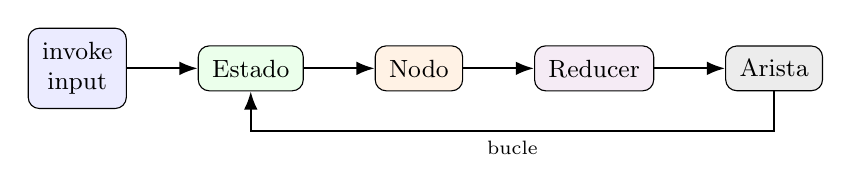
\begin{tikzpicture}[
  box/.style={draw, rounded corners, align=center, font=\small, inner sep=5pt},
  arr/.style={-{Latex}, thick}
]
\node[box, fill=blue!8] (inv) {invoke\\input};
\node[box, fill=green!8, right=0.9cm of inv] (st) {Estado};
\node[box, fill=orange!10, right=0.9cm of st] (nd) {Nodo};
\node[box, fill=violet!8, right=0.9cm of nd] (mg) {Reducer};
\node[box, fill=gray!15, right=0.9cm of mg] (nx) {Arista};
\draw[arr] (inv) -- (st);
\draw[arr] (st) -- (nd);
\draw[arr] (nd) -- (mg);
\draw[arr] (mg) -- (nx);
\draw[arr] (nx.south) -- ++(0,-0.5) -| node[pos=0.25, below, font=\scriptsize]{bucle} (st.south);
\end{tikzpicture}
\end{center}

Vocabulario mínimo:
\begin{itemize}[leftmargin=*,itemsep=1pt]
  \item \textbf{State}: TypedDict / schema con campos.
  \item \textbf{Node}: \texttt{state $\to$ update} (dict parcial).
  \item \textbf{Edge}: fija o condicional (router).
  \item \textbf{Reducer}: cómo se fusiona update + estado (p.\,ej.\ \texttt{add\_messages}).
  \item \textbf{Compile}: congela el grafo en un Runnable (\texttt{invoke}/\texttt{stream}).
  \item \texttt{START}/\texttt{END}: entrada/salida.
\end{itemize}

% =============================================================================
\section{Receta: montar un grafo desde cero}
\label{sec:recipe}
% =============================================================================

\begin{howto}[title=Checklist (cópiala cuando construyas uno nuevo)]
\begin{enumerate}[leftmargin=*,itemsep=2pt]
  \item \textbf{Define el estado}: ¿historial de mensajes o campos (\texttt{question}, \texttt{documents},\ldots)?
  \item \textbf{Lista los nodos}: cada uno hace \emph{una} cosa (reason, act, grade,\ldots).
  \item \textbf{Dibuja las aristas}: fijas vs ``si X entonces Y''.
  \item \textbf{Criterio de parada}: ¿sin tool\_calls? ¿contador? ¿grader dice useful?
  \item \textbf{Implementa nodos} que \texttt{return \{campo: valor\_nuevo\}}.
  \item \texttt{StateGraph(...)} $\to$ \texttt{add\_node} $\to$ entry $\to$ edges $\to$ \texttt{compile()}.
  \item \texttt{invoke} con la shape correcta del estado inicial.
  \item Dibuja el grafo (\texttt{draw\_mermaid}) para validar el diseño.
\end{enumerate}
\end{howto}

\begin{fromcode}[title=Esqueleto genérico]
\begin{lstlisting}
from langgraph.graph import StateGraph, START, END

builder = StateGraph(MyState)
builder.add_node("a", node_a)
builder.add_node("b", node_b)
builder.add_edge(START, "a")                 # o set_entry_point("a")
builder.add_conditional_edges("a", router, {"b": "b", END: END})
builder.add_edge("b", "a")                   # bucle
app = builder.compile()
result = app.invoke({...})                   # keys = campos del estado
\end{lstlisting}
\end{fromcode}

% =============================================================================
\section{Mensajes (agentes de chat)}
\label{sec:messages}
% =============================================================================

En 01--03 la conversación es una \textbf{lista tipada}, no un string.

\begin{center}
\begin{tabular}{@{}llp{7.6cm}@{}}
\toprule
\textbf{Clase} & \textbf{Rol} & \textbf{Para qué} \\
\midrule
\texttt{HumanMessage} & user & Pregunta / feedback ``como usuario'' \\
\texttt{AIMessage} & assistant & Texto y/o \texttt{tool\_calls} \\
\texttt{SystemMessage} & system & Reglas (a menudo inyectadas en el nodo) \\
\texttt{ToolMessage} & tool & Resultado real (\texttt{tool\_call\_id} obligatorio) \\
\bottomrule
\end{tabular}
\end{center}

\subsection{Ciclo tool-calling (obligatorio recordarlo)}
\begin{enumerate}[leftmargin=*,itemsep=1pt]
  \item \texttt{HumanMessage}
  \item \texttt{AIMessage} con \texttt{tool\_calls} --- el modelo \emph{pide} (no ejecuta)
  \item \texttt{ToolMessage}(s) --- tu código / \texttt{ToolNode} ejecuta
  \item nuevo \texttt{AIMessage} --- final o más tool\_calls
\end{enumerate}

\begin{warn}[title=bind\_tools $\neq$ ejecutar]
\texttt{bind\_tools} enseña el schema. Quien ejecuta es \texttt{ToolNode} (o tu nodo manual).
Sin nodo act, el AIMessage con tool\_calls queda colgado.
\end{warn}

\begin{howto}[title=Arrancar un grafo de mensajes]
\begin{lstlisting}
res = app.invoke({
    "messages": [HumanMessage(content="What is the weather in Tokyo?")]
})
# o dicts: {"messages": [{"role": "user", "content": "..."}]}
print(res["messages"][-1].content)
\end{lstlisting}
\end{howto}

% =============================================================================
\section{Estado y reducers}
\label{sec:state}
% =============================================================================

\subsection{Regla de oro}
El nodo \textbf{devuelve un update parcial}, no reescribe el mundo entero:

\begin{lstlisting}
return {"messages": [response]}   # "añade esto"
\end{lstlisting}

\subsection{\texttt{add\_messages}}
\begin{concept}[title=Reducer de chat]
\texttt{Annotated[list, add\_messages]} fusiona listas:
por defecto \textbf{append}; si el mensaje nuevo tiene el mismo \texttt{id}, \textbf{reemplaza}.
Por eso basta devolver solo el mensaje nuevo.
\end{concept}

Dos formas equivalentes:

\begin{center}
\begin{tabular}{@{}p{7.4cm}p{7.4cm}@{}}
\toprule
\textbf{Atajo (01, 03)} & \textbf{Explícito (02)} \\
\midrule
\begin{lstlisting}
from langgraph.graph import MessagesState
StateGraph(MessagesState)
\end{lstlisting}
&
\begin{lstlisting}
class MessageGraph(TypedDict):
    messages: Annotated[
        list[BaseMessage], add_messages]
\end{lstlisting}
\\
\bottomrule
\end{tabular}
\end{center}

\begin{warn}[title=Sin reducer = overwrite]
\texttt{messages: list[...]} sin \texttt{Annotated[..., add\_messages]}
suele \textbf{pisar} el historial y romper tool calling.
\end{warn}

\subsection{Estado \emph{sin} mensajes (04)}
Cuando el flujo no es un chat sino un pipeline de datos:

\begin{lstlisting}
class GraphState(TypedDict):
    question: str
    generation: str
    web_search: bool
    documents: List[str]   # en la práctica: List[Document]
\end{lstlisting}

Aquí cada update \textbf{sobrescribe} el campo (last-value). Eso es correcto:
no quieres ``append'' de la pregunta; quieres el valor actual.

\begin{lookup}[title=¿MessagesState o TypedDict custom?]
¿El LLM necesita historial de turnos/tools? $\to$ mensajes + \texttt{add\_messages}.
¿Orquestas retrieve/grade/generate con flags? $\to$ campos explícitos (04).
¿Ambos? $\to$ mezcla: \texttt{messages} anotado + otros campos.
\end{lookup}

% =============================================================================
\section{Nodos, aristas, ToolNode}
\label{sec:flow}
% =============================================================================

\subsection{Contrato de un nodo}
\begin{lstlisting}
def my_node(state: MyState) -> dict:
    # lee state["..."]
    # calcula
    return {"campo": nuevo_valor}   # solo lo que cambió
\end{lstlisting}

Puede encapsular LCEL (\texttt{prompt | llm}), retrieval, HTTP, etc.

\subsection{Aristas}
\begin{center}
\begin{tabular}{@{}p{7.2cm}p{7.6cm}@{}}
\toprule
\textbf{Fija} & \textbf{Condicional} \\
\midrule
\texttt{add\_edge("act", "reason")}
siempre act $\to$ reason
&
\texttt{add\_conditional\_edges(src, router, mapping)}
router mira estado $\to$ clave del mapping
\\
\bottomrule
\end{tabular}
\end{center}

\begin{howto}[title=Router típico tras un LLM con tools]
\begin{lstlisting}
def should_continue(state: MessagesState) -> str:
    if not state["messages"][-1].tool_calls:
        return END
    return "act"
\end{lstlisting}
\end{howto}

Variantes de mapping:
\begin{itemize}[leftmargin=*,itemsep=1pt]
  \item Dict: \texttt{\{END: END, "act": "act"\}}
  \item Lista de destinos: \texttt{["execute\_tools", END]} (03) si el router ya devuelve el nombre del nodo
\end{itemize}

\subsection{Entry points}
\begin{itemize}[leftmargin=*,itemsep=1pt]
  \item \texttt{set\_entry\_point("draft")} o \texttt{add\_edge(START, "draft")}
  \item \texttt{set\_conditional\_entry\_point(router, \{...\})} --- la \emph{primera} decisión depende del input (04: vectorstore vs web)
\end{itemize}

\subsection{\texttt{ToolNode}}
\begin{lstlisting}
from langgraph.prebuilt import ToolNode
tool_node = ToolNode(tools)
\end{lstlisting}
Lee el último \texttt{AIMessage}, ejecuta cada \texttt{tool\_call}, emite \texttt{ToolMessage}s.

\begin{tip}[title=Nombre de la tool = nombre del tool\_call]
En 03 las ``tools'' se registran con \texttt{name=AnswerQuestion.\_\_name\_\_}
para que coincidan con lo que el LLM pide vía \texttt{bind\_tools}.
\end{tip}

% =============================================================================
\section{Módulo 01 --- ReAct en grafo}
\label{sec:react}
% =============================================================================

\begin{concept}[title=Idea]
Reason + Act en bucle. El LLM razona (y pide tools); el grafo actúa; se vuelve a razonar con resultados en el historial.
\end{concept}

\begin{center}
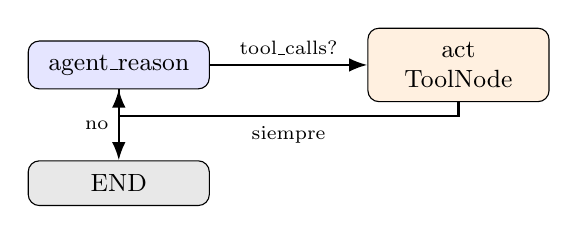
\begin{tikzpicture}[
  n/.style={draw, rounded corners, align=center, font=\small, inner sep=5pt, minimum width=2.3cm},
  arr/.style={-{Latex}, thick}
]
\node[n, fill=blue!10] (r) {agent\_reason};
\node[n, fill=orange!12, right=2.0cm of r] (a) {act\\ToolNode};
\node[n, fill=gray!18, below=0.9cm of r] (e) {END};
\draw[arr] (r) -- node[above, font=\scriptsize]{tool\_calls?} (a);
\draw[arr] (r) -- node[left, font=\scriptsize]{no} (e);
\draw[arr] (a) -- ++(0,-0.65) -| node[pos=0.25, below, font=\scriptsize]{siempre} (r);
\end{tikzpicture}
\end{center}

\subsection{Archivos}
\begin{itemize}[leftmargin=*,itemsep=1pt]
  \item \texttt{react.py}: \texttt{TavilySearch} + \texttt{triple} + \texttt{llm.bind\_tools(tools)}
  \item \texttt{nodes.py}: \texttt{run\_agent\_reasoning} + \texttt{ToolNode}
  \item \texttt{main.py}: grafo, \texttt{should\_continue}, invoke
\end{itemize}

\subsection{Qué viaja en el estado (ejemplo)}
\begin{enumerate}[leftmargin=*,itemsep=1pt]
  \item invoke: \texttt{[Human(...)]}
  \item reason $\to$ append \texttt{AIMessage(tool\_calls=[...])}
  \item router $\to$ act $\to$ append \texttt{ToolMessage}s
  \item reason de nuevo (ya ve resultados) $\to$ más tools o texto final
  \item sin \texttt{tool\_calls} $\to$ END
\end{enumerate}

\begin{howto}[title=Reutiliza este patrón cuando\ldots]
\ldots{}necesites un agente clásico ``usa tools hasta responder''.
Copia: \texttt{MessagesState} + nodo LLM con \texttt{bind\_tools} + \texttt{ToolNode} + conditional edge por \texttt{tool\_calls}.
Cambia solo la lista de tools y el system prompt.
\end{howto}

\begin{fromcode}[title=nodes.py --- reason añade un AIMessage]
\begin{lstlisting}
def run_agent_reasoning(state: MessagesState):
    response = llm.invoke(
        [{"role": "system", "content": SYSATEM_MESSAGE}, *state["messages"]]
    )
    return {"messages": [response]}
\end{lstlisting}
\end{fromcode}

\begin{tip}
El system prompt se inyecta en el invoke del nodo (no se guarda en el estado).
Así no ensucias el historial persistente.
\end{tip}

% =============================================================================
\section{Módulo 02 --- Reflection}
\label{sec:reflect}
% =============================================================================

\begin{concept}[title=Idea]
Dos roles: \textbf{generate} escribe; \textbf{reflect} critica; generate revisa.
El ``acto'' es criticar texto, no una tool externa.
\end{concept}

\begin{center}
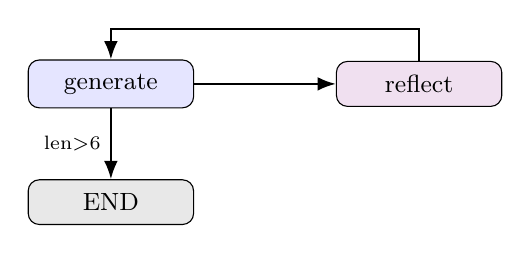
\begin{tikzpicture}[
  n/.style={draw, rounded corners, align=center, font=\small, inner sep=5pt, minimum width=2.1cm},
  arr/.style={-{Latex}, thick}
]
\node[n, fill=blue!10] (g) {generate};
\node[n, fill=violet!12, right=1.8cm of g] (r) {reflect};
\node[n, fill=gray!18, below=0.9cm of g] (e) {END};
\draw[arr] (g) -- (r);
\draw[arr] (r) -- ++(0,0.7) -| (g);
\draw[arr] (g) -- node[left, font=\scriptsize]{len$>$6} (e);
\end{tikzpicture}
\end{center}

\subsection{LCEL como cerebro del nodo}
\begin{lstlisting}
generation_prompt = ChatPromptTemplate.from_messages([
    ("system", "You write excellent twitter posts..."),
    MessagesPlaceholder(variable_name="messages"),
])
generate_chain = generation_prompt | llm
\end{lstlisting}

\texttt{MessagesPlaceholder} inyecta \textbf{todo} el historial: request + drafts + críticas.

\subsection{Truco clave del reflector}
\begin{lstlisting}
def reflection_node(state):
    res = reflect_chain.invoke({"messages": state["messages"]})
    return {"messages": [HumanMessage(content=res.content)]}
\end{lstlisting}

La crítica se guarda como \texttt{HumanMessage} para que el generador la trate como feedback externo
(no como ``él mismo hablando otra vez'').

\subsection{Parada}
\begin{lstlisting}
def should_continue(state):
    if len(state["messages"]) > 6:
        return END
    return REFLECT
\end{lstlisting}

\begin{howto}[title=Reutiliza Reflection cuando\ldots]
\ldots{}quieras mejorar un artefacto (tweet, email, código) con un crítico.
Necesitas: dos prompts, dos nodos, edge reflect$\to$generate, conditional generate$\to$END|reflect, y un contador/heurística de parada.
\end{howto}

% =============================================================================
\section{Módulo 03 --- Reflexion (research loop)}
\label{sec:reflexion}
% =============================================================================

\begin{concept}[title=Idea]
Más potente que Reflection:
(1)~draft estructurado con auto-crítica y search queries,
(2)~ejecutar esas queries (Tavily),
(3)~revisar con citas,
(4)~repetir hasta $N$ iteraciones.
\end{concept}

\begin{center}
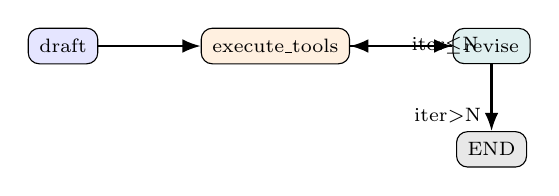
\begin{tikzpicture}[
  n/.style={draw, rounded corners, align=center, font=\scriptsize, inner sep=4pt},
  arr/.style={-{Latex}, thick}
]
\node[n, fill=blue!10] (d) {draft};
\node[n, fill=orange!12, right=1.3cm of d] (t) {execute\_tools};
\node[n, fill=teal!12, right=1.3cm of t] (r) {revise};
\node[n, fill=gray!18, below=0.85cm of r] (e) {END};
\draw[arr] (d) -- (t);
\draw[arr] (t) -- (r);
\draw[arr] (r) -- node[right, font=\scriptsize]{iter$\le$N} (t);
\draw[arr] (r) -- node[below left, font=\scriptsize]{iter$>$N} (e);
\end{tikzpicture}
\end{center}

\subsection{Schemas Pydantic = ``tools'' de salida}
\begin{lstlisting}
class AnswerQuestion(BaseModel):
    answer: str
    reflection: Reflection      # missing / superfluous
    search_query: List[str]     # 1-3 queries

class ReviseAnswer(AnswerQuestion):
    references: List[str]
\end{lstlisting}

El LLM no llama Tavily directamente: emite un \texttt{AnswerQuestion} vía tool calling;
luego \texttt{ToolNode} ejecuta \texttt{run\_queries(search\_queries)}.

\begin{howto}[title=Forzar el schema]
\begin{lstlisting}
first_responder = prompt | llm.bind_tools(
    tools=[AnswerQuestion], tool_choice="AnswerQuestion"
)
\end{lstlisting}
\texttt{tool\_choice} obliga a usar esa tool (salida estructurada fiable).
\end{howto}

\subsection{ToolNode con nombres alineados}
\begin{lstlisting}
execute_tools = ToolNode([
    StructuredTool.from_function(run_queries, name=AnswerQuestion.__name__),
    StructuredTool.from_function(run_queries, name=ReviseAnswer.__name__),
])
\end{lstlisting}

\subsection{Parada por contador de ToolMessages}
\begin{lstlisting}
def event_loop(state) -> Literal["execute_tools", END]:
    num_iterations = sum(isinstance(m, ToolMessage) for m in state["messages"])
    if num_iterations > MAX_ITERATIONS:  # 2 en el curso
        return END
    return "execute_tools"
\end{lstlisting}

\begin{howto}[title=Reutiliza Reflexion cuando\ldots]
\ldots{}necesites investigación con evidencia: draft $\to$ search $\to$ revise $\to$ cite.
Piezas: Pydantic answer+critique+queries, \texttt{bind\_tools}+\texttt{tool\_choice}, ToolNode que ejecuta searches, MAX\_ITERATIONS.
\end{howto}

\begin{tip}[title=Leer la respuesta final]
Tras \texttt{invoke}, el último mensaje suele ser un \texttt{AIMessage} con tool\_calls;
la respuesta tipada está en \texttt{tool\_calls[0]["args"]["answer"]}.
\end{tip}

% =============================================================================
\section{Módulo 04 --- Agentic RAG}
\label{sec:rag}
% =============================================================================

\begin{concept}[title=Idea]
RAG clásico + decisiones:
¿vectorstore o web? ¿docs relevantes? ¿la respuesta está grounded? ¿responde la pregunta?
Si falla, busca en la web o regenera.
\end{concept}

\subsection{Estado (campos, no chat)}
\begin{lstlisting}
class GraphState(TypedDict):
    question: str
    generation: str
    web_search: bool
    documents: List[...]
\end{lstlisting}

Entrada típica: \texttt{app.invoke(\{"question": "What is film noir?"\})}.

\subsection{Nodos}
\begin{center}
\begin{tabular}{@{}lp{10.5cm}@{}}
\toprule
\textbf{Nodo} & \textbf{Qué hace} \\
\midrule
\texttt{retrieve} & \texttt{retriever.invoke(question)} $\to$ documents \\
\texttt{grade\_documents} & LLM grader por doc; filtra; pone \texttt{web\_search} si hay irrelevantes \\
\texttt{web\_search} & Tavily $\to$ Document; lo añade a documents \\
\texttt{generate} & \texttt{prompt | llm | StrOutputParser} con context + question \\
\bottomrule
\end{tabular}
\end{center}

\subsection{Flujo (intención del diseño)}
\begin{enumerate}[leftmargin=*,itemsep=1pt]
  \item \textbf{Router de entrada}: film noir / Bogart $\to$ retrieve; otro tema $\to$ web\_search
        (\texttt{set\_conditional\_entry\_point} + \texttt{RouteQuery}).
  \item retrieve $\to$ grade\_documents.
  \item Si docs flojos (\texttt{web\_search=True}) $\to$ web\_search; si no $\to$ generate.
  \item Tras generate: hallucination grader + answer grader:
        \begin{itemize}[leftmargin=*,itemsep=0pt]
          \item useful $\to$ END
          \item not useful $\to$ WEB\_SEARCH
          \item not supported $\to$ GENERATE de nuevo
        \end{itemize}
  \item web\_search $\to$ generate (siempre).
\end{enumerate}

\begin{howto}[title=Structured output para routers/graders]
\begin{lstlisting}
class RouteQuery(BaseModel):
    datasource: Literal["vectorstore", "web_search"] = Field(...)

router = prompt | llm.with_structured_output(RouteQuery)
source = router.invoke({"question": q})
# source.datasource == "vectorstore" | "web_search"
\end{lstlisting}
Igual para graders binarios (\texttt{binary\_score}, \texttt{is\_hallucinated}).
\end{howto}

\subsection{Ingestión (una vez)}
\texttt{ingestion.py}: URLs film noir $\to$ UnstructuredLoader $\to$ RecursiveSplitter (250/20)
$\to$ \texttt{OllamaEmbeddings(nomic-embed-text)} $\to$ Chroma (\texttt{collection\_name="film-noir"}).
El \texttt{retriever} se importa en el nodo retrieve.

\begin{howto}[title=Reutiliza Agentic RAG cuando\ldots]
\ldots tu corpus es parcial y quieres fallback a web + auto-chequeo de calidad.
Necesitas: estado con question/documents/generation/flags, nodos retrieve/grade/search/generate,
y 2--3 chains de grading con \texttt{with\_structured\_output}.
\end{howto}

\begin{warn}[title=Detalle del repo]
En \texttt{graph.py} aparecen \texttt{set\_entry\_point(RETRIEVE)} y
\texttt{set\_conditional\_entry\_point(...)}. Si ambos están, comprueba cuál queda activo
en tu versión de LangGraph; el diseño didáctico apunta al router condicional.
Además, al gradear docs conviene comparar \texttt{score.binary\_score == "yes"}
(objeto Pydantic), no el objeto entero con el string \texttt{"yes"}.
\end{warn}

% =============================================================================
\section{Patrones: cuándo usar cuál}
\label{sec:patterns}
% =============================================================================

\begin{center}
\begin{tabular}{@{}p{3.2cm}p{5.5cm}p{6.5cm}@{}}
\toprule
\textbf{Patrón} & \textbf{Cuándo} & \textbf{Esencia} \\
\midrule
ReAct & Tools externas, pregunta abierta & reason $\leftrightarrow$ ToolNode hasta sin tool\_calls \\
Reflection & Mejorar un draft con crítica & generate $\leftrightarrow$ reflect; crítica como Human \\
Reflexion & Research + citas + mejora & draft(struct) $\to$ search $\to$ revise; $N$ iters \\
Agentic RAG & Corpus + fallback + QA check & route / grade / search / regenerate \\
\bottomrule
\end{tabular}
\end{center}

\begin{tip}[title=LangGraph vs \texttt{create\_agent}]
\texttt{create\_agent} oculta el bucle.
LangGraph te deja \textbf{diseñar} cuándo tools, cuándo criticar, cuándo buscar web, qué guardar en estado.
\end{tip}

% =============================================================================
\section{Cheat sheet ultra-corta}
\label{sec:cheatsheet}
% =============================================================================

\begin{center}
\begin{tabular}{@{}p{5.0cm}p{10.2cm}@{}}
\toprule
\textbf{Idea} & \textbf{Recuerda} \\
\midrule
Crear grafo & \texttt{StateGraph(State)} $\to$ nodes $\to$ edges $\to$ \texttt{compile()} \\
Entrada chat & \texttt{\{"messages": [HumanMessage(...)]\}} \\
Entrada RAG & \texttt{\{"question": "..."\}} \\
Salida de nodo & \texttt{return \{"campo": valor\}} (parcial) \\
Historial seguro & \texttt{MessagesState} / \texttt{add\_messages} \\
LLM + tools & \texttt{.bind\_tools(tools)} \\
Ejecutar tools & \texttt{ToolNode(tools)} \\
¿Seguir (ReAct)? & \texttt{state["messages"][-1].tool\_calls} \\
Schema forzado & \texttt{tool\_choice="Nombre"} o \texttt{with\_structured\_output} \\
Historial en prompt & \texttt{MessagesPlaceholder("messages")} \\
Parar & mapear a \texttt{END} \\
Ver flujo & \texttt{get\_graph().draw\_mermaid\_png(...)} \\
\bottomrule
\end{tabular}
\end{center}

% =============================================================================
\section{Errores mentales frecuentes}
\label{sec:pitfalls}
% =============================================================================

\begin{enumerate}[leftmargin=*,itemsep=2pt]
  \item Devolver el historial completo a mano con \texttt{add\_messages}: innecesario; solo el mensaje nuevo.
  \item Olvidar el reducer $\to$ pisas mensajes.
  \item Confundir \texttt{tool\_calls} (pedir) con ejecutar.
  \item No volver al LLM tras \texttt{ToolMessage}.
  \item Reflection/Reflexion sin tope de iteraciones $\to$ bucle infinito.
  \item ToolNode cuyo \texttt{name} no coincide con el del schema Pydantic.
  \item Mezclar embedding distinto en ingest vs retrieve (04: \texttt{nomic-embed-text}).
  \item Invocar 04 sin haber corrido \texttt{ingestion.py} (Chroma vacío).
  \item Esperar \texttt{messages} en Agentic RAG: aquí el contrato es \texttt{question}/\texttt{generation}/\ldots
\end{enumerate}

% =============================================================================
\section{Guía archivo por archivo}
% =============================================================================

\begin{longtable}{@{}p{5.6cm}p{9.6cm}@{}}
\toprule
\textbf{Archivo} & \textbf{Qué aprender} \\
\midrule
\endhead
\texttt{01/.../react.py} & Tools + \texttt{bind\_tools} \\
\texttt{01/.../nodes.py} & Nodo reason; \texttt{ToolNode} \\
\texttt{01/.../main.py} & Grafo ReAct completo + router \\
\texttt{02/.../chains.py} & Dos LCEL chains (generate/reflect) \\
\texttt{02/.../main.py} & Estado custom + crítica como HumanMessage \\
\texttt{03/.../schemas.py} & AnswerQuestion / ReviseAnswer / Reflection \\
\texttt{03/.../chains.py} & \texttt{tool\_choice} + prompts actor/revisor \\
\texttt{03/.../tool\_executor.py} & ToolNode + Tavily batch queries \\
\texttt{03/.../main.py} & draft $\to$ tools $\to$ revise + event\_loop \\
\texttt{04/.../ingestion.py} & Crawl URLs $\to$ Chroma \\
\texttt{04/.../graph/state.py} & Estado por campos \\
\texttt{04/.../graph/nodes/*} & retrieve / grade / web / generate \\
\texttt{04/.../graph/chains/*} & router + graders + generation \\
\texttt{04/.../graph/graph.py} & Wiring + conditional entry + self-correct \\
\texttt{04/.../main.py} & \texttt{app.invoke(\{"question": ...\})} \\
\bottomrule
\end{longtable}

% =============================================================================
\section{Glosario}
% =============================================================================

\begin{center}
\begin{tabular}{@{}p{4.2cm}p{11cm}@{}}
\toprule
\textbf{Término} & \textbf{En la práctica} \\
\midrule
State & Memoria compartida del grafo \\
Node & Función que propone un update \\
Edge / conditional & Transición fija / con router \\
Reducer & Política de merge (\texttt{add\_messages}, overwrite\ldots) \\
ToolNode & Ejecuta tool\_calls $\to$ ToolMessages \\
ReAct & Bucle razonar--actuar \\
Reflection & Generar--criticar--revisar (texto) \\
Reflexion & Draft estructurado + search + revise \\
Agentic RAG & RAG con routing, grading y reintentos \\
Structured output & Pydantic vía tools o \texttt{with\_structured\_output} \\
Checkpointer & Persistencia entre pasos/runs (avanzado; no en estos módulos) \\
\bottomrule
\end{tabular}
\end{center}

\vspace{1em}
\begin{center}
\fbox{\parbox{0.92\textwidth}{\centering
\textbf{Frase resumen}\\[0.35em]
\textit{Diseña el estado, escribe nodos que devuelven parches,}\\
\textit{conecta aristas (condicionales cuando haya decisiones),}\\
\textit{compila e invoca. El patrón (ReAct / Reflection / Reflexion / RAG)}\\
\textit{solo cambia qué nodos y qué criterios de parada usas.}
}}
\end{center}

\vspace{0.8em}
\noindent\textit{Compilar:} \texttt{pdflatex langgraph-resumen.tex} (dos veces para TOC estable).

\end{document}
